\section{Introduction}\label{s:intro}

\TODO{
This section includes some motivations behind the work, explicitly or implicitly
highlights the research question, provides a high-level explanation of the
solution, and describes the contributions.
}


\lipsum[1-2]

\begin{figure}[bh]
    %% The macro `\onecolgrid' is defined in `vusec.sty'
    %% NOTE: The suffix "./figs/" is implicitly included for this relative path.
    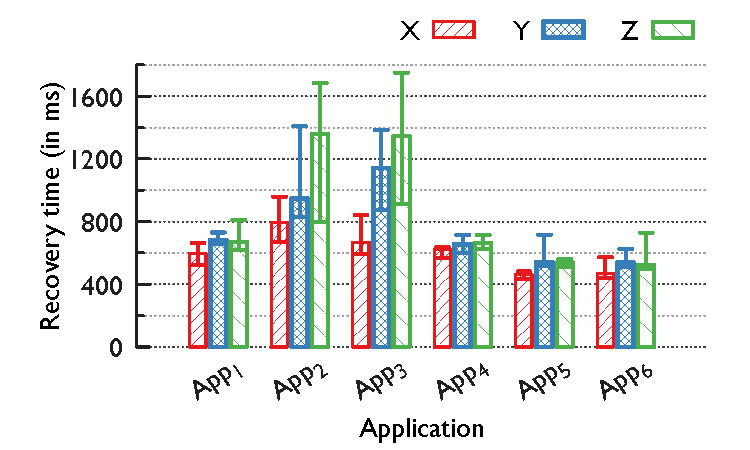
\includegraphics[width=\onecolgrid]{cache-by-app}
    %% Labels should immediately follow caption, to keep latex quiet.
    \figcap{Simple one-column figure. Please include a brief explanation or
    takeaway.}\label{fig:1col}
\end{figure}

\lipsum[3-4]

\begin{figure*}[th]
    %% The macro `\threecolgrid' is defined in `vusec.sty'
    \begin{subfigure}[t]{\threecolgrid}
        %% NOTE: The suffix "./figs/" is implicitly included for these relative paths.
        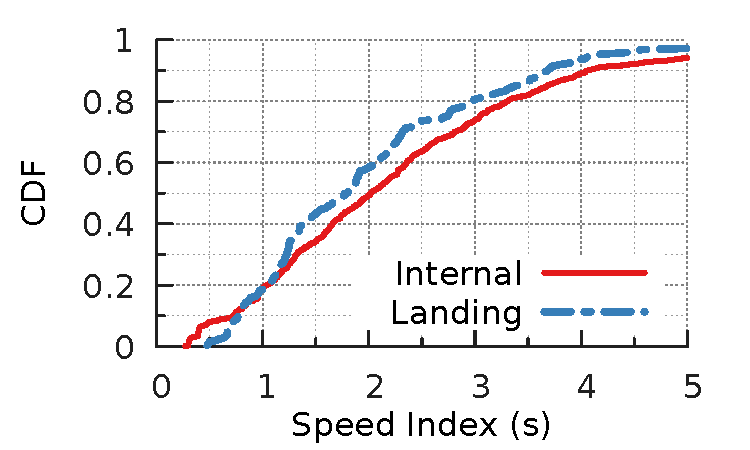
\includegraphics[width=\linewidth]{three-col/speed_index}
        \sfigcap{}\label{fig:3col-a}
    \end{subfigure}
    \begin{subfigure}[t]{\threecolgrid}
        %% NOTE: You do not have to mention the extension.
        %% (The example figures are in PDF format.)
        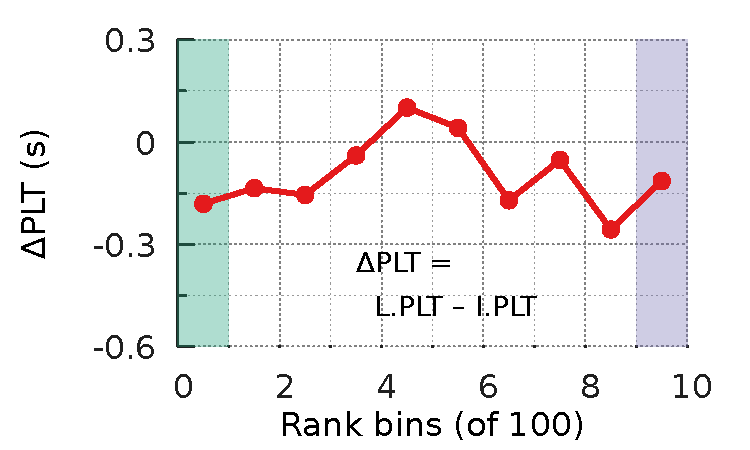
\includegraphics[width=\linewidth]{three-col/plt_ranks_diff}
        \sfigcap{}\label{fig:3col-b}
    \end{subfigure}
    \begin{subfigure}[t]{\threecolgrid}
        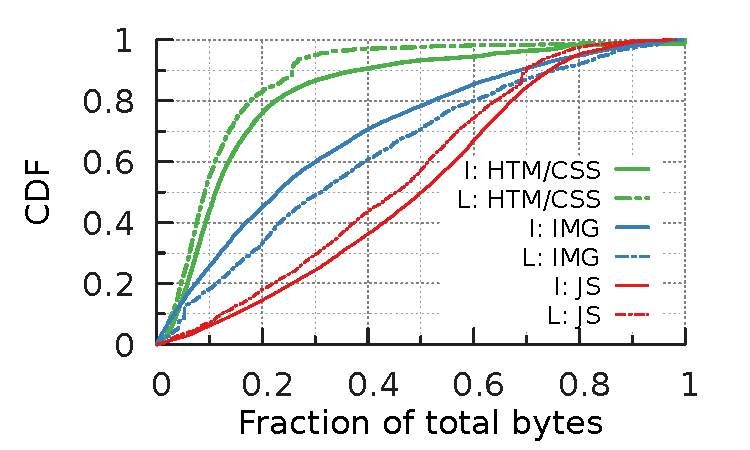
\includegraphics[width=\linewidth]{three-col/mimes}
        \sfigcap{}\label{fig:3col-c}
    \end{subfigure}
    %% Labels should immediately follow caption, to keep latex quiet.
    \figcap{Generate clear and beautiful figures (in PDF) that can be rendered side by side while still being easy to read and interpret. Choose colors wisely from the colorbrewer2.org website.}\label{fig:3col}
\end{figure*}

\lipsum[6-8]

\begin{table}[hb]
    \centering
    \tabcap{A simple table describing the characteristics of a data set or the
    results of an experiment.}\label{tab:sample}
    \taburulecolor{black!45}
    \begin{tabu}{c|c|r|r|r|r}
        \toprule
        \multirow{2}{*}{\thead{Char.}} &
            \multirow{2}{*}{\thead{\#samples}} &
            \thead{Count} &
            \multicolumn{3}{c}{\thead{Perf. Score}}\\
        &
            &
            \thead{of items} &
            \thead{X} & \thead{Y} & \thead{Z} \\
        \midrule
        \stress{P}
            & 214 & 56 & 9 & 23 & 24 \\
        \stress{Q}
            & 117 & 27 & 7 & 10 & 10 \\
        \stress{R}
            & 222 & 11 & 6 & 4 & 1 \\
        \stress{S}
            & 187 &  9 & 1 & 6 & 2 \\
        \stress{T}
            & 180 & 16 & 7 & 5 & 4 \\
        \bottomrule
    \end{tabu}

\end{table}

\lipsum[12-18]

\TODO{
We summarize our contributions as follows.
}

\case{}
%
\lipsum[10][1-2]

\case{}
% 
\lipsum[11][3-4]

\case{}
% 
\lipsum[12][5-6]


%%% Local Variables:
%%% mode: latex
%%% TeX-master: "../thesis"
%%% End:
